% =========================
% Project Documentation
% =========================

\section{Project documentatie}
\label{sec:project-documentatie}

\subsection{Inleiding}
\label{sec:project-documentatie-inleiding}

In dit hoofdstuk wordt er gekeken naar hoe de individuele samenvattingen van een Python bestand gebruikt kunnen worden om een samenvatting van het gehele project te maken.
Alsook wordt er verder gekeken naar hoe de relaties tussen de verschillende bestanden gevisualiseerd kunnen worden.
Dit om een zo goed mogelijk overzicht te krijgen van het project, zonder dat er handmatig documentatie moet worden geschreven.

\subsection{Projectsamenvatting}
\label{sec:project-documentatie-samenvatting}

De samenvatting van een Python project kan gemaakt worden door de individuele samenvattingen van de bestanden samen te voegen.
Deze samenvatting kan bekomen worden door elk python bestand in het project te laten documenteren en de samenvatting ervan op te slaan.
Erna kunnen deze samenvattingen samengevoegd worden om dan mee te geven aan een Large Language Model.
Deze samenvattingen worden gegenereerd door het aanroepen van de functie \mintinline{python3}|generate_file_summaries()|. 
Deze functie maakt gebruik van de klasse \mintinline{python3}|FileDocumenationGenerator()| die de samenvattingen van de bestanden genereerd en opslaat in een dictionary.
De code van deze functie is te vinden in \ref{bijlage:file-summary-functions}.  

Door een duidelijk prompt mee te geven aan het model, kan er specifiek gevraagd worden welke functies en klassen er in het project zitten en dat per bestand duidelijk opgelijst. Samen met deze oplijsting wordt er ook een korte samenvatting van het gehele project weergegeven.
Een voorbeeld van de uitkomst is te zien in \ref{fig:project-summary}.
Hier is te zien dat er een duidelijk overzicht is van welke functies en klassen er in het project zitten, alsook wat het gehele project inhoudt.

\begin{figure}[h]
    \centering
    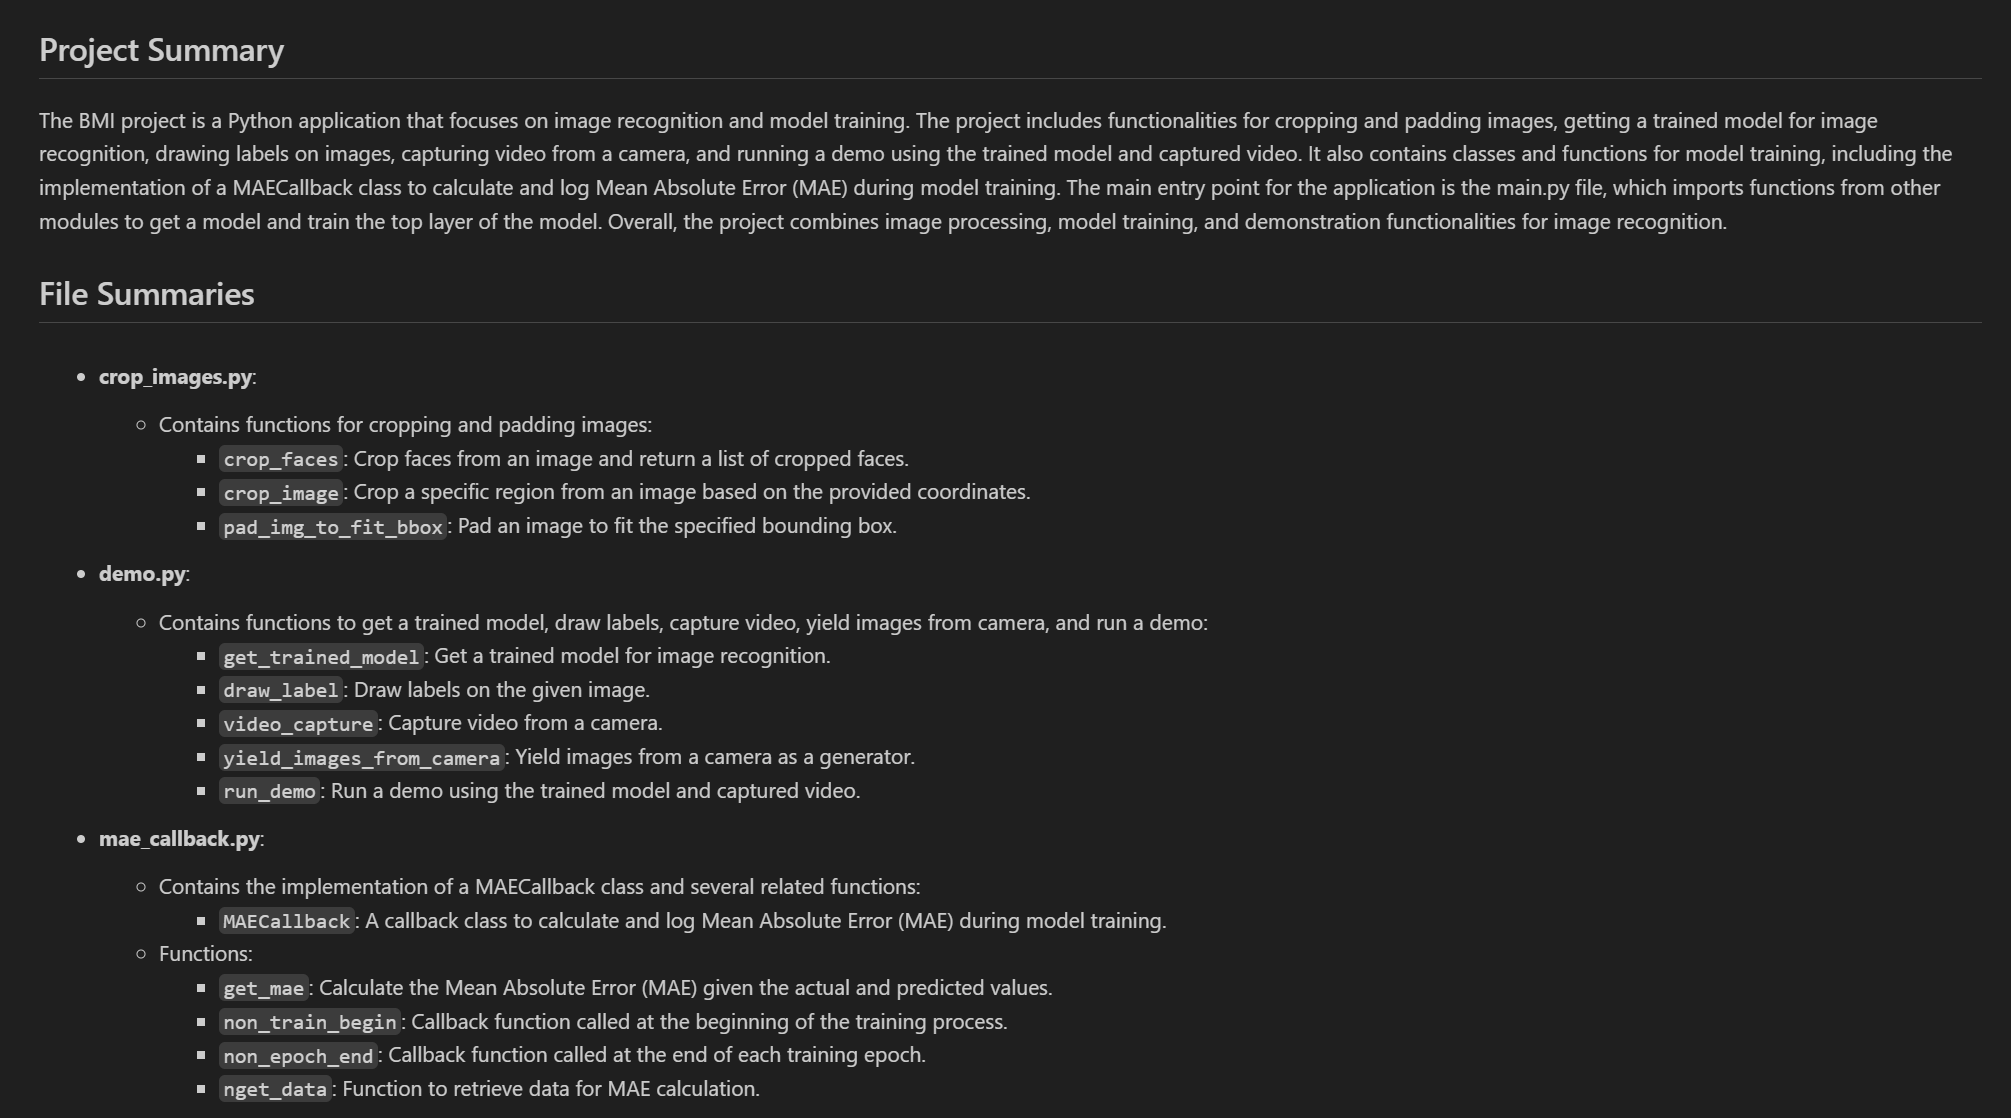
\includegraphics[width=1\textwidth]{project_summary.png}
    \caption{Voorbeeld van een project samenvatting}
    \label{fig:project-summary}
\end{figure}    

\subsubsection{Keuze van welke bestanden te documenteren}
\label{subsec:project-documentatie-keuze-bestanden}

Het is belangrijk om te kijken naar welke bestanden er gedocumenteerd moeten worden.
Omdat het gaat over een Python project, is het belangrijk dat alle Python bestanden gedocumenteerd worden.
Er is de keuze gemaakt om het bestand \mintinline{python3}|__init__.py| niet te documenteren, omdat dit bestand vaak niet relevant is voor de documentatie van het project.
Dit omdat het bestand vaak leeg is of slechts minimale functionaliteit bevat. 
Ook bevat het soms enkele configuratie opties die niet relevant zijn voor de documentatie.

\subsubsection{Documentatie van bestanden zonder functies of klassen}
\label{subsec:project-documentatie-geen-functies}

Omdat er eerst vanuit gegaan wordt dat elk bestand functies of klassen bevat, is het belangrijk om te kijken naar bestanden die dit niet bevatten.
Deze bestanden dienen ook gedocumenteerd te worden om een volledig overzicht te krijgen van het project.
Als er geen apart prompt voorzien wordt dan zal het model hallucineren en een samenvatting verzinnen, dit is niet de bedoeling.
Er is gebruik gemaakt van een prompt \ref{bijlage:bestand-zonder-functies} die vraagt om de werking van het document uit te leggen en de eventuele imports die het bestand bevat.
In dit prompt wordt er duidelijk gedefinieerd wat er in de documentatie moet staan. 
En aan de hand van een voorbeeld wordt er getoond hoe de documentatie eruit moet zien.
Een voorbeeld van de uitkomst in de project documentatie van een bestand zonder functies is te zien in \ref{fig:file-no-functions}.

\begin{figure}[h]
    \centering
    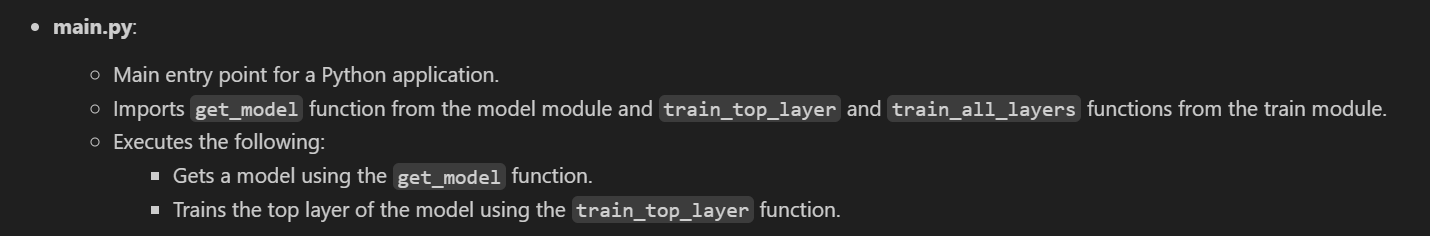
\includegraphics[width=1\textwidth]{documentatie_bestand_zonder_functies.png}
    \caption{Voorbeeld van de documentatie van een bestand zonder functies of klassen}
    \label{fig:file-no-functions}
\end{figure}

\subsubsection{Prompting voor projectsamenvatting}
\label{sec:project-documentatie-prompting}

Aangezien de samenvatting van een project bestaat uit de samenvattingen van individuele Python bestanden, is het belangrijk dat deze op een correcte manier gegenereerd worden.
Dit wordt gerealiseerd met behulp van een prompt die de samenvatting van een Pythonbestand op een correcte manier interpreteert en omzet naar de juiste documentatie.

De gehele samenvatting van het project werd gemaakt door de individuele samenvattingen van de bestanden samen te voegen en dit mee te geven met het prompt \ref{bijlage:prompt6}.
De volgorde van de samenvattingen is niet van belang, omdat de relaties tussen de bestanden later nog gevisualiseerd worden en dit op basis van de imports \ref{sec:project-documentatie-relaties}.
Dit prompt vraagt om de samenvatting van het project te maken en uit de individuele samenvattingen de functies en klassen op te lijsten.

Hierdoor was het niet mogelijk om de gewenste samenvatting te creëren door alle individuele samenvattingen mee te geven aan het model.
Een oplossing die gevonden werd is de volgende: er werden verschillende kleinere prompts meegegeven met het model.
Dit prompt maakt per samenvatting van een Python bestand de documentatie van de verschillende functies en klassen. 
De functies en klassen worden opgelijst met het juiste formaat en een kleine uitleg.
Deze resultaten van de verschillende kleine prompts werden dan code matig samengevoegd tot een geheel. 
Er gaat niets verloren van de individuele samenvattingen, maar om de samenvattingen per bestand met eenzelfde opmaak te krijgen, is deze oplossing gekozen.
Een LLM begrijpt beter een kleiner prompt dan een groot prompt, omdat het model dan beter kan focussen op de vraag en een beter antwoord kan geven.
De uitkomst van de samenvatting van het project is te zien in \ref{fig:project-summary}.

Het prompt dat gebruikt werd is te zien in \ref{bijlage:prompt7}.
Dit prompt vraagt om de functies en klassen van een Python bestand op te lijsten en een korte uitleg te geven van wat deze functies en klassen doen.
De uitkomst is weergegeven met een duidelijk voorbeeld binnen het prompt en volgens een markdown formaat. 
De documentatie genereerd door dit prompt is te zien in \ref{fig:project-summary}.

\subsection{Visualisatie van relaties tussen bestanden}
\label{sec:project-documentatie-relaties}

Om een goed overzicht te krijgen van het project is het belangrijk om de relaties tussen de verschillende bestanden te visualiseren.
Dit kan gedaan worden door gebruik te maken van graven om de relaties tussen de bestanden weer te geven.
Omdat er uit de longlist is gebleken dat er een bestaande tool is die dit kan, namelijk \textcite{Doxygen2023}, is deze tool grondig bekeken.
Voordat Doxygen een visualisatie maakt van de relaties tussen de bestanden vergen deze bestanden grondige documentatie, de relaties tussen de bestanden dienen toegevoegd worden.
Doordat deze tool documentatie vergt, is er gekeken naar hoe deze relaties gegenereerd kunnen worden met behulp van LLM's.
Ook is er gekeken naar hoe Doxygen deze relaties visualiseert, er wordt binnen \textcite{Doxygen2023} gebruikt gemaakt van \textcite{GraphvizAuthors2024}.

\textcite{GraphvizAuthors2024} kan niet gebruikt worden in een Python omgeving, de taal waarin dit onderzoek geschreven is.
Daarom is er gekeken naar een alternatief en soortgelijke tool om de relaties te weergeven.
De tool Pyvis van \textcite{WHIR2018} is een Python library die te gebruiken is om graven te maken en te visualiseren.
Dit laat het toe om de relaties tussen de verschillende bestanden te visualiseren en een duidelijk overzicht te krijgen van het project.

\subsubsection{Genereren van de relaties tussen bestanden in een project}
\label{subsec:project-documentatie-relaties-genereren}

Om de relaties te bekomen tussen alle bestanden en mappen in een project is er een prompt meegegeven aan het Large Language Model.
In dit prompt worden de imports van alle bestanden opgelijst en wordt er gevraagd om de relaties tussen de bestanden weer te geven.
Omdat een bestand dat een functie uit een ander bestand gebruikt deze functie importeerd, staat deze ook tussen de verschillende imports van het bestand.
Hierdoor kan er gekeken worden naar de imports van de verschillende bestanden en zo kunnen de relaties tussen de bestanden worden gevisualiseerd.

Het prompt dat gebruikt werd is te zien in bijlage \ref{bijlage:generate-file-relations}.
Er zijn verschillende iteraties van dit prompt gemaakt om de beste resultaten te bekomen.
Deze iteraties en fouten in het prompt hebben enige tijd in beslag genomen om op te lossen, maar uiteindelijk zijn de kinderziektes eruit gehaald.
Zo is het belangrijk dat er geen spaties in het voorbeeld CSV staan, omdat het model dan niet de het juiste CSV bestand kan genereren.
Ook is het belangrijk dat de imports van de bestanden correct zijn, omdat het model anders niet de juiste relaties kan genereren. 
De uitkomst van dit prompt is een CSV bestand met daarin het pad van het bestand, de bestandsnaam, het pad van de folder waarin het bestand zit en een lijst van alle geimporteerde bestanden.
Omdat dit CSV bestand de basis is voor de graaf die later gemaakt wordt, is het belangrijk dat dit bestand correct is.
Ook zijn schrijffouten en onduidelijkheden in het prompt aangepast om een beter resultaat te bekomen.

Een verdere iteratie van het prompt laat het toe om alle imports in het CSV te laten staan, er wordt achteraf gefilterd op de imports die niet relevant zijn.
Ook is er duidelijk gemaakt aan het prompt dat het bij meerdere imports deze moet opslaan in een lijst gescheiden met een puntkomma.

\subsubsection{Visualisatie van de relaties}
\label{subsec:project-documentatie-relaties-visualisatie}

Eens er een goed CSV bestand is bekomen kunnen de relaties tussen de bestanden gevisualiseerd worden.
Dit wordt gedaan met behulp van de tool Pyvis \autocite{WHIR2018}.
Deze tool haalt de relaties uit het CSV bestand en voegt deze toe aan een graaf. 
Dit door eerst de verschillende nodes toe te voegen en dan de edges tussen de nodes. 
De code waarop dit gebeurt is te vinden in bijlage \ref{bijlage:generate-file-graph}.
Als dit voor alle bestanden gedaan is, kan er een duidelijk overzicht bekomen worden van de relaties tussen de bestanden door de graaf te exporteren naar een HTML bestand.
Dit HTML bestand kan dan geopend worden in een browser om de graaf te bekijken, alsook kunnen de nodes versleept worden om een beter overzicht te bekomen.

\begin{figure}[h]
    \centering
    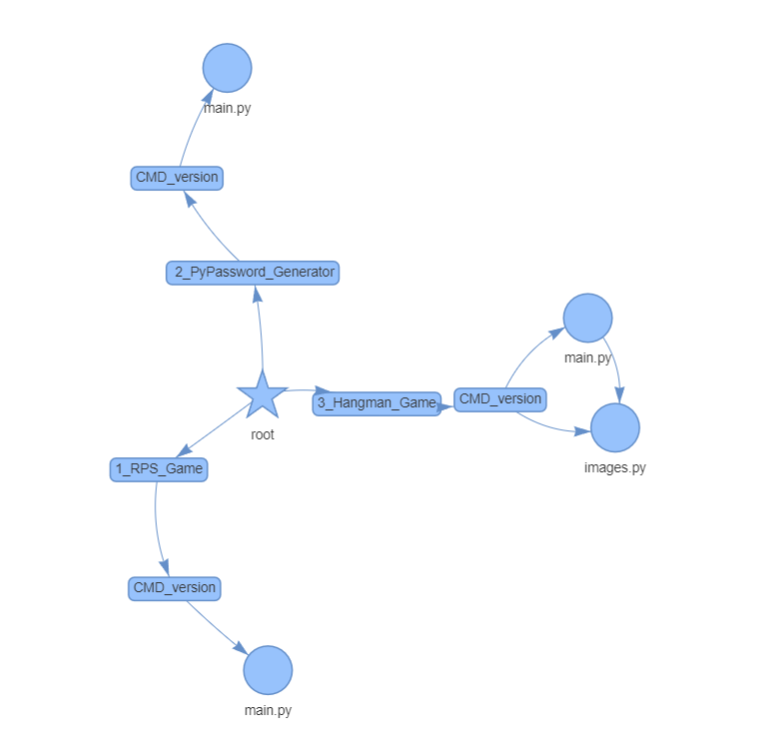
\includegraphics[width=0.5\textwidth]{graph.png}
    \caption{Voorbeeld van een graaf van de relaties tussen bestanden}
    \label{fig:graph}
\end{figure}

Er is een voorbeeld van een graaf te zien in \ref{fig:graph}, alsook is er een voor een groot project een graaf gemaakt om te kijken of de relaties tussen de bestanden duidelijk weergegeven worden op grote schaal \ref{fig:graph-large}.
De relaties op deze graaf zijn zichtbaar echter is het niet altijd duidelijk omdat er veel bestanden zijn en er bepaalde bestanden vaak geïmporteerd zijn.
Dit kan ervoor zorgen dat de graaf onoverzichtelijk wordt met de mate de grote van het projectOpenAi.

\begin{figure}[h]
    \centering
    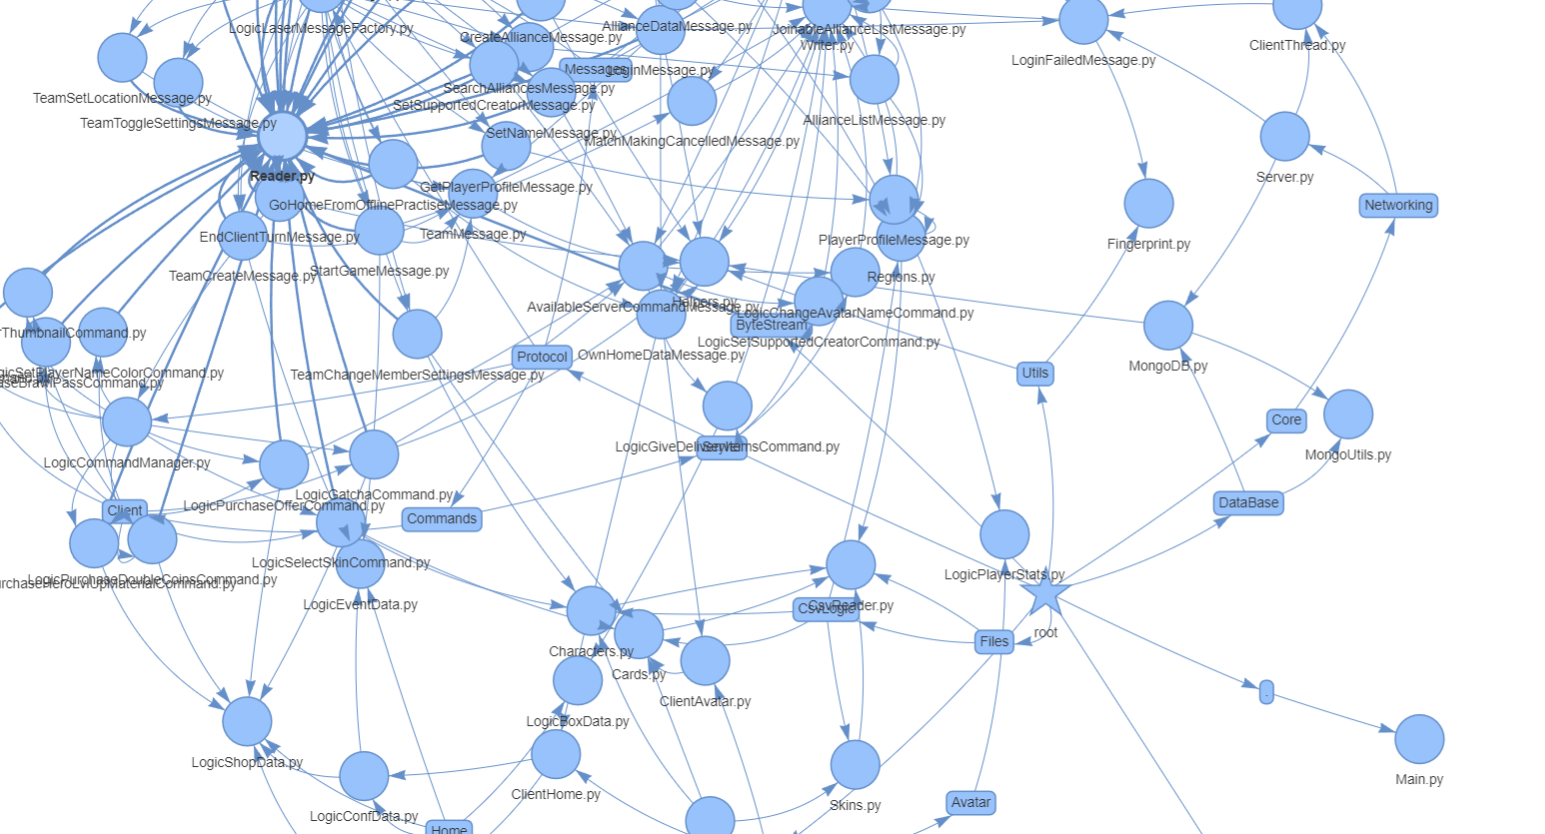
\includegraphics[width=1\textwidth]{graph-large.png}
    \caption{Voorbeeld van een fragment van een graaf van de relaties tussen bestanden van een groot project}
    \label{fig:graph-large}
\end{figure}

\section{Evaluatie}
\label{sec:project-documentatie-evaluatie}

\subsection{Inleiding}
\label{sec:project-documentatie-evaluatie-inleiding}

In dit hoofdstuk wordt er gekeken naar hoe de documentatie van een project geëvalueerd kan worden.
Dit wordt gedaan door de documentatie van de tool te vergelijken met de handgeschreven documentatie van een project.
Dit voor een Python bestand genaamd AutoClicker van \textcite{Waegeneer2022} en een Python project met de naam bmi-project van \textcite{Simmons2019}.

\subsection{Bestanddocumentatie evaulatie}
\label{sec:project-documentatie-evaluatie-bestand}

Door het testen van de moeilijkheidgraden opgesteld in \ref{table:bestanden} kon de tool geëvalueerd worden.
De tool werkte zoals verwacht voor bestanden met moeilijkheidsgraad makkelijk tot moeilijk.
Het vergelijken van de zelfgedocumenteerde bestanden met de automatisch gegenereerde bestanden geeft een goed beeld van de kwaliteit van de gegenereerde docstrings en bestandsamenvattingen.
Wat te zien is in \ref{fig:evaluatie-bestand-documentatie}.
Hieruit is te zien dat de functie omschrijvingen in de samenvatting anders verwoord zijn, maar de betekenis is hetzelfde.
Er is echter één functie die niet gedocumenteerd is manueel, die wel gedocumenteerd is door de tool.
Dit toont aan dat de tool beter presteert dan de programmeur zelf.
Dit is een goed resultaat, omdat de gegenereerde docstrings correct zijn en de samenvatting een correct beeld geeft van het bestand.

\begin{figure}
    \centering
    \begin{subfigure}[b]{1\textwidth}
        \centering
        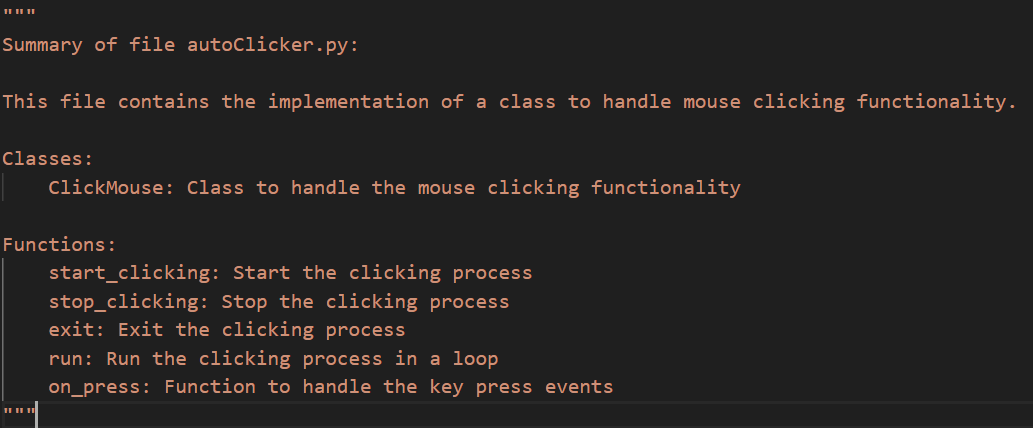
\includegraphics[width=1\textwidth]{zelf_autoclick.png}
        \caption{Zelfgedocumenteerde bestandsamenvatting. \ref{bijlage:zelfgedocumenteerd-bestand}}
        \label{fig:zelfgedocumenteerd-bestandsamenvatting}
    \end{subfigure}
    \hfill
    \begin{subfigure}[b]{1\textwidth}
        \centering
        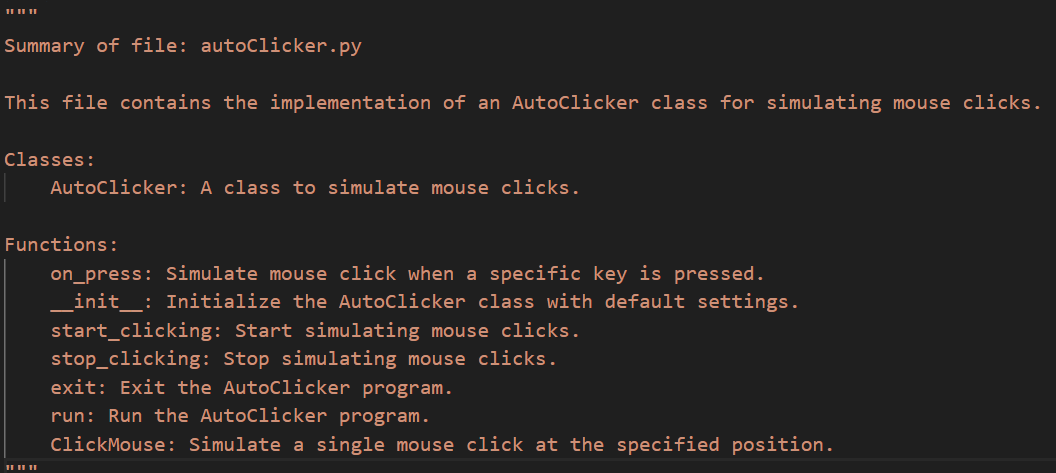
\includegraphics[width=1\textwidth]{automatisch_autoclick.png}
        \caption{Automatisch gegenereerde bestandsamenvatting van eigen tool. \ref{bijlage:evaluatie-bestand-documentatie}}
        \label{fig:automatisch-bestandsamenvatting}
    \end{subfigure}
    \caption{Evaluatie van de automatisch gegenereerde bestandsamenvatting met de zelfgedocumenteerde bestandsamenvatting. Voor het bestand AutoClicker van \textcite{Waegeneer2022}}
    \label{fig:evaluatie-bestand-documentatie}
\end{figure}


\subsection{projectdocumentatie evaluatie}
\label{sec:project-documentatie-evaluatie-project}

Er is een Pythonprojecthandmatig gedocumenteerd, aan dit project zijn de docstrings toegevoegd, samenvattingen per bestand en een samenvatting van het gehele project.
De visualisatie tussen de verschillende bestanden is getekend op papier.

\begin{figure}
    \centering
    \begin{subfigure}[b]{1\textwidth}
        \centering
        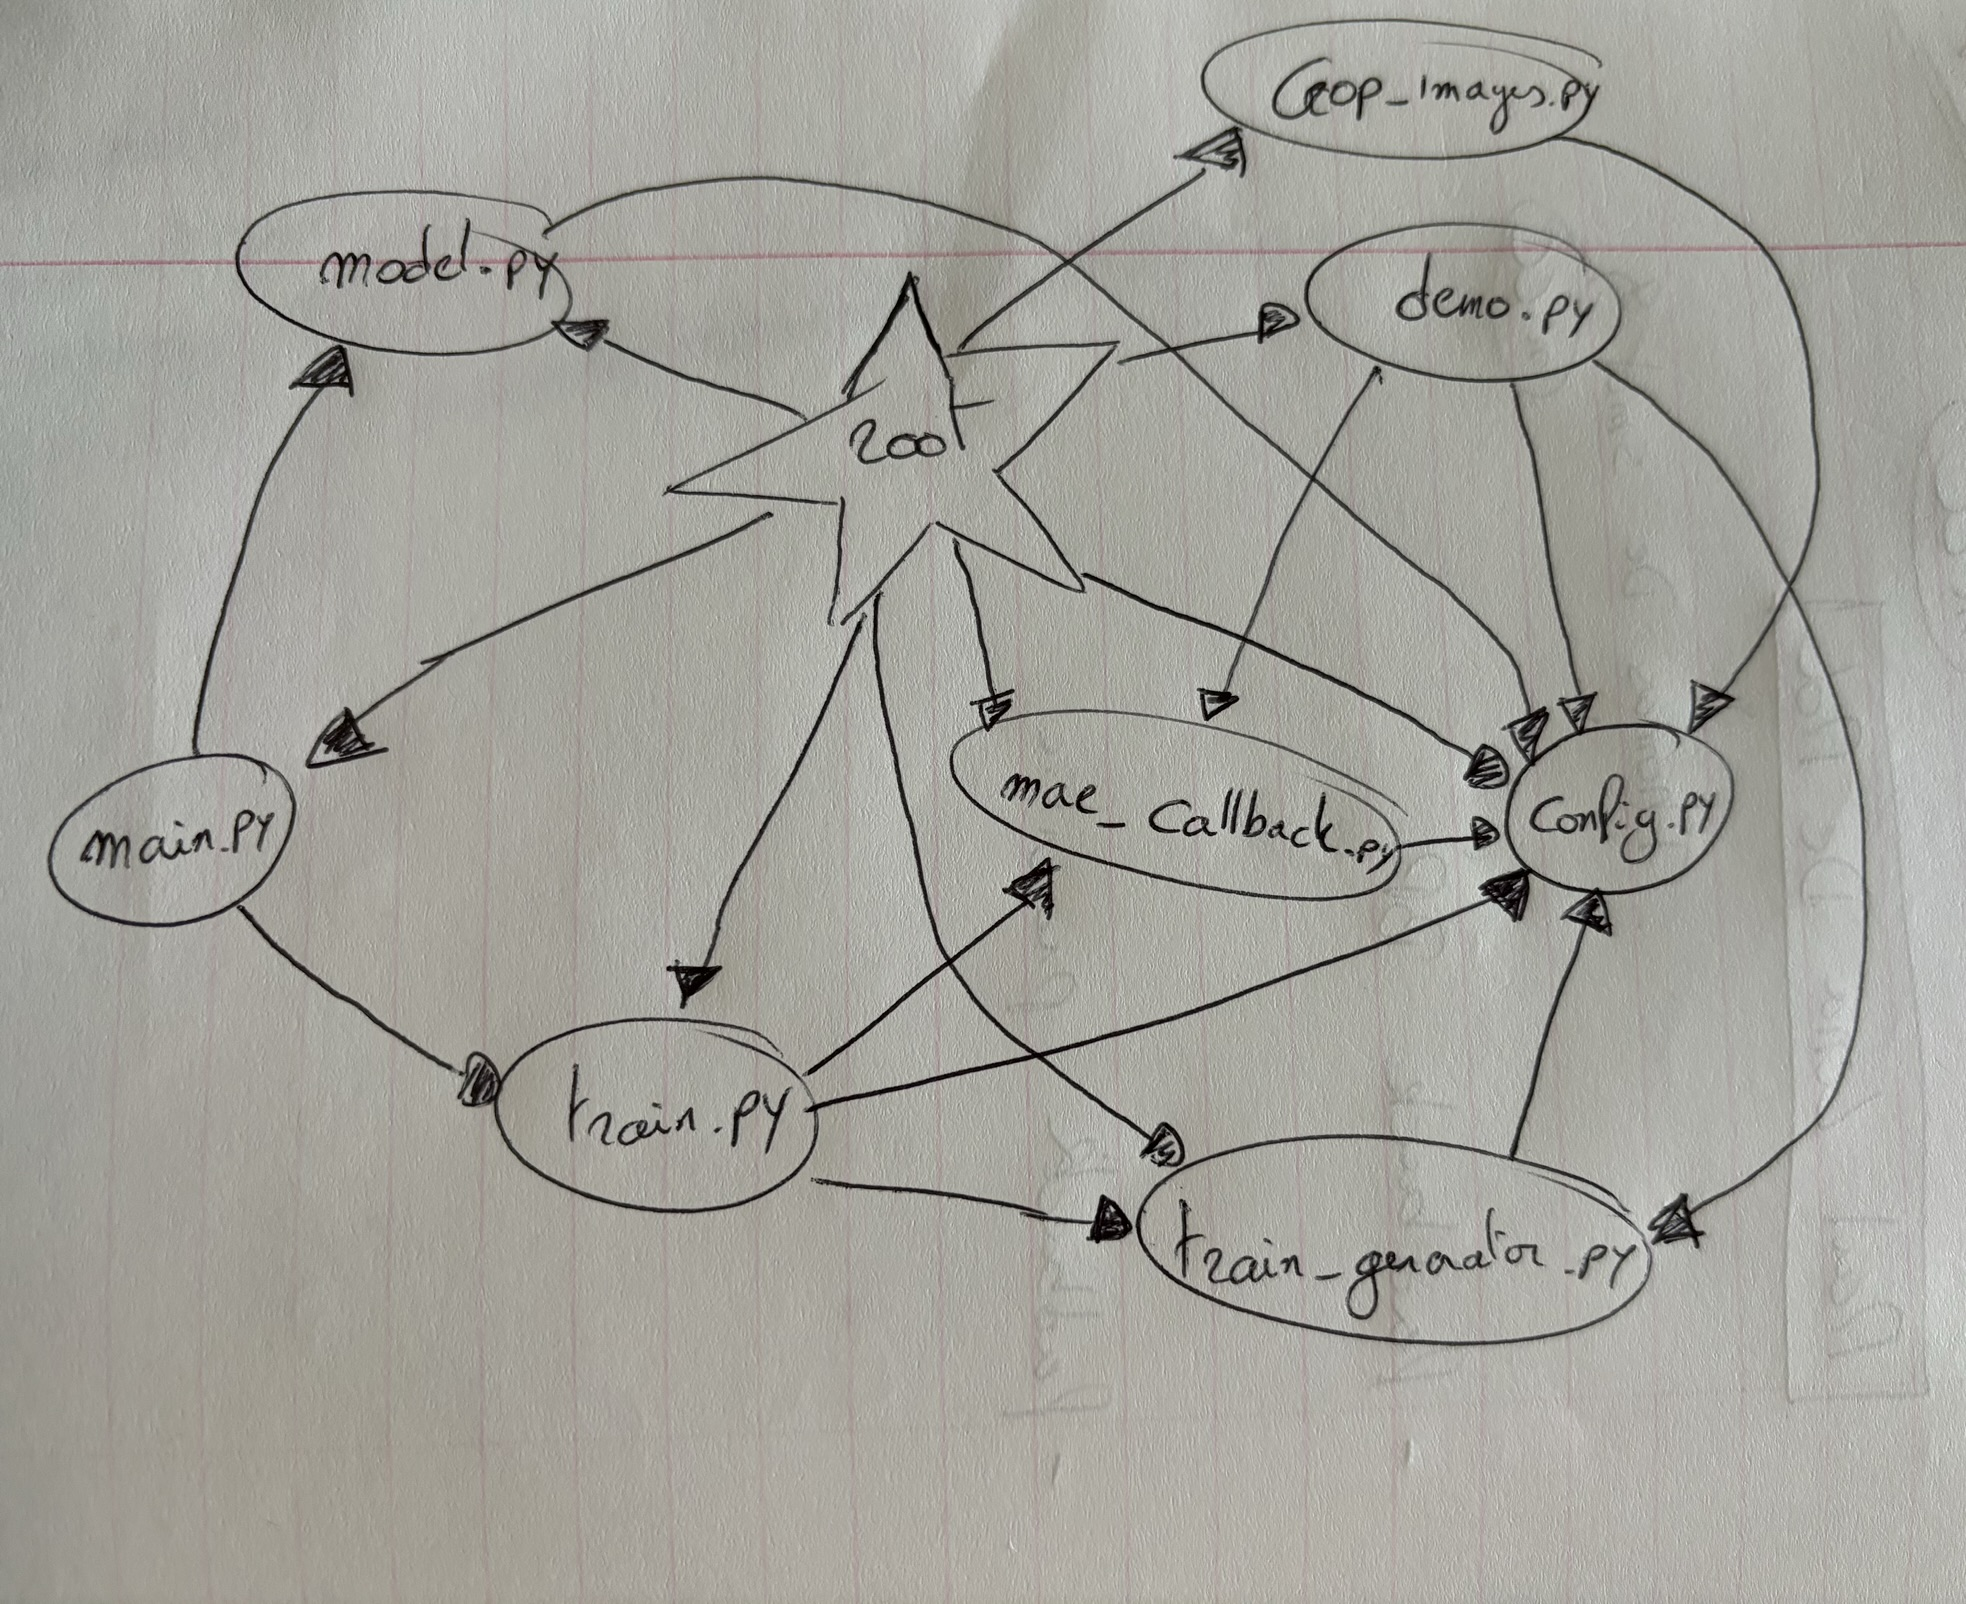
\includegraphics[width=0.5\textwidth]{graaf.png}
        \caption{Handgetekende graaf van de relaties tussen de bestanden van het project \autocite{Simmons2019}}
    \end{subfigure}
    \hfill
    \begin{subfigure}[b]{0.5\textwidth}
        \centering
        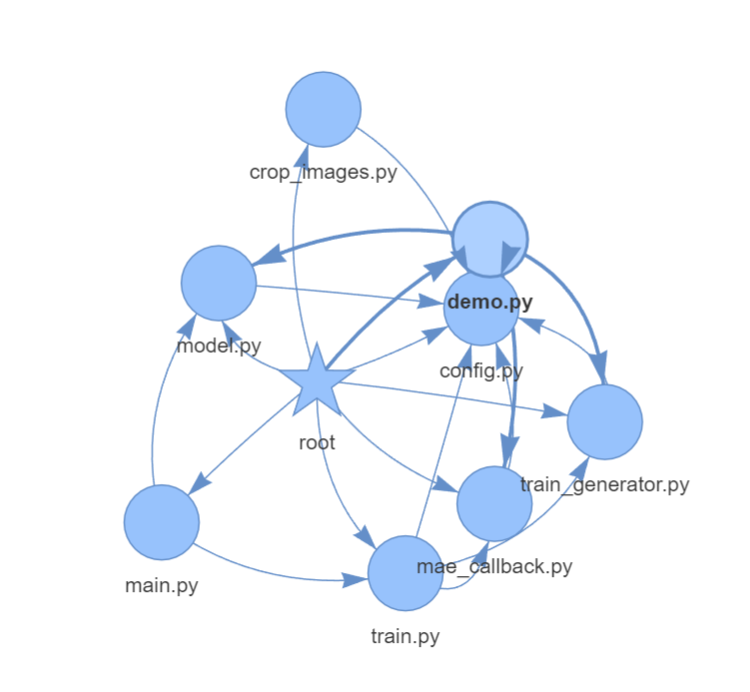
\includegraphics[width=1\textwidth]{generated_graaf.png}
        \caption{Gegenereerde graaf van de relaties tussen de bestanden van het project. \autocite{Simmons2019}}
    \end{subfigure}
    \caption{Vergelijking van de gegenereerde graaf met de handgetekende graaf.}
    \label{fig:evaluatie-graaf}
\end{figure}

De graven te zien in \ref{fig:evaluatie-graaf} tonen de relaties tussen de bestanden van het project. 
Het is duidelijk dat deze graven gelijkaardig zijn, de gegenereerde graaf is beweegbaar en kan aangepast worden om een beter overzicht te krijgen.

Het vergelijken van de samenvattingen en de docstrings laat blijken dat de gegenereerde documentatie correct is.

